\documentclass{article}
\usepackage[a4paper, margin=1in]{geometry}
\usepackage{graphicx}
\usepackage{hyperref}
\usepackage{polski}
\usepackage{float}

\title{Sztuczna inteligencja i inżyniera wiedzy\\
        Sprawozdanie z laboratorium 1}
\author{Patryk Łuszczek \\
        Numer indeksu: 272707
        \\ Grupa 1}
\date{\today}

\begin{document}

\maketitle

\section{Zadanie 1}
\subsection*{Graf i wprowadzenie danych}
W celu zrealizowania zadania, został stworzony graf na podstawie danych dostarczonych w ramach zadania.
Grał bazuje na implementacji grafu wielokrotnie skierowanego z biblioteki NetworkX i rozszerza go o dodatkowe funkcjonalności takie jak np. znajdowanie najlepszego połączenia z uwzględnieniem zmiennych kryteriów, oraz normalizacją
danych przy ich ładowaniu. Wierzchołek reprezentuje pojedynczy przystanek wraz z jego danymi geolokacyjnymi. W celu uproszczenia, przystanki o tej samej nazwie są traktowane jako jeden wierzchołek, czas podróży oraz odległości między takimi przystankammi były na tyle niewielkie,
że nie wpłwa to na jakość działania algorytmów.

\begin{figure}
    \centering
    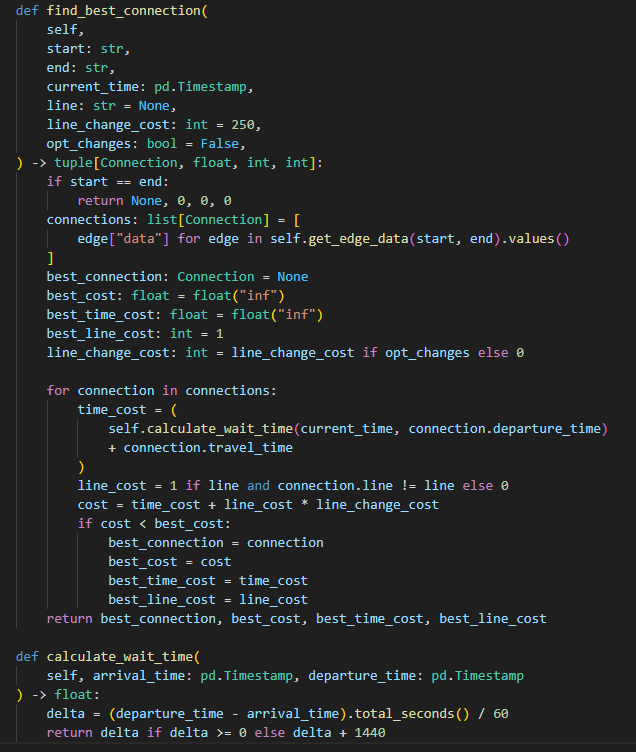
\includegraphics[width=0.5\textwidth]{sc1.png}
\end{figure}

Została utworzona dataklasa \texttt{Connection} reprezentująca połączenia w grafie, która zawiera niezbędne informacje tj. linia oraz czas podróży.

\begin{figure}[H]
    \centering
    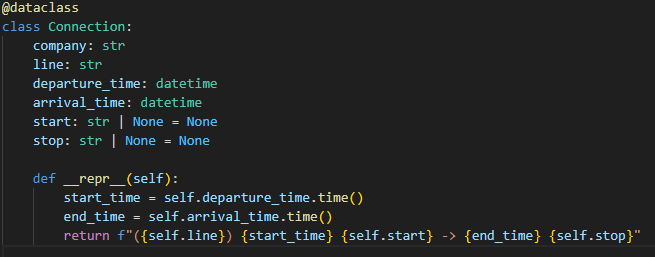
\includegraphics[width=0.5\textwidth]{sc2.png}
\end{figure}



\subsection*{Algortytm Dijkstry}
Algorytm Dijkstry służy do znajdowania najkrótszej ścieżki. Opiera się na kolejce priorytetowej, w której znajdują się następne wierzchołki do odwiedzenia, a ułożone są według wyliczonych wcześniej wag. Początkowo 
znajduje się w niej wyłącznie wierzchołek początkowy o wadze równej zero, następnie odwiedzane są sąsiednie wierzchołki, a ich wagi są ustalane jako waga wierzchołka, z którego zostały odwiedzone oraz waga krawędzi, tj. połączenia. Z racji, że 
między dwoma wierzchołkami może występować wiele krawędzi, wybierana jest ta najlepsza, zgodnie z kryterium optymalizacji, tutaj czasem podróży. Następnie wierzchołek jest dodawany do kolejki, a algorytm działa dopóki
nie dotrze do wierzchołka docelowego lub kolejka nie będzie pusta. W momencie dotarcia do wierzchołka docelowego, algorytm kończy działanie i zwraca najkrótszą ścieżkę oraz czas podróży.


\subsection*{Algorytm A*}
Algorytm A* jest również algorytmem służącym do znajdowania najkrótszej ścieżki, jednak w odróżnieniu od Dijkstry wykorzystuje dodatkowo heurystykę,
która umożliwia szacowanie pozostałego kosztu dla danego węzła. Dzięki temu, algorytm może działać szybciej, jednak rozwiązanie może nie zawsze być optymalne.
Jako heurystykę wykorzystałem obliczenie pozostałęgo czasu podróży na podstawie danych lokalizacyjnych przystanków. W przypadku moich algorytmów, implementacyjnie A* niewiele różni się od Dijkstry, z wyjątkiem wykorzystania właśnie dodatkowego kroku 
obliczenia heurystyki.

\begin{figure}[H]
    \centering
    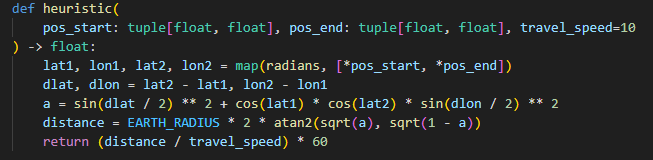
\includegraphics[width=0.5\textwidth]{sc3.png}
\end{figure}

Oba algorytmy wykorzystują funkcję kosztu polegającą na obliczeniu czasu oczekwiania na dotarcie do przystanku, uwzględniając czas podróży oraz czas oczekiwania na polączenie. Dodatkowo, jeśli 
optymalizowana jest liczba przesiadek, to kara za przesiadkę jest dodawana do całkowitego kosztu.

\subsection*{Wnioski}
Dla przykłądowych danych testowych tj:
\begin{verbatim}
    start = 'Metalowców'
    end = 'Pl. Grunwaldzki'
    time = '12:00:00'
\end{verbatim}


Dodatkowo, na tej samej trasie została wykorzystana opcja optymalizacji liczby przesiadek dla algorytmu A*.



\section{Zadanie 2}
Do implementacji tabu search, wykorzsystałem działanie algorytmu A*, który porównuje koszt dla różnych kombinacji przystanków do odwiedzenia. 
Tablica tabu jest dobierana na podstawie liczby przystanków do odwiedzenia, a sąsiedztwo oraz jego rozmiar jest obliczany na podstawie zmian kolejności w odniesieniu do obcnego rozwiązania.
Dodatkowo, jeśli od kilku iteracji nie znaleziono lepszego rozwiązania, to przeszukiwane jest większe sąsiedztwo. Wykorzystana została również aspiracja, która pozwala na
zignorowanie tabu. Wartość aspiracji jest ustalana na podstawie obecnie najlepszego kosztu, oraz wartości zmian jakie zachodziły w poprzednich iteracjach.

Dla przykłądowych danych testowych tj:
\begin{verbatim}
    start = 'Psie Pole'
    end = 'Śliczna'
    time = '12:00:00'
    stops = ['Piastowska','Most Grunwaldzki','Galeria Dominikańska',' 'Pl. Wróblewskiego','Dworzec Główny]
\end{verbatim}




\end{document}
